\documentclass[../main.tex]{subfiles}
\ifSubfilesClassLoaded{\setcounter{chapter}{2}}{}
\begin{document}

\chapter{Pengenalan Algoritma dan Flowchart}

\begin{subcpmk}
  \item Sub-CPMK 1.1: Menjelaskan definisi dan fungsi flowchart
  \item Sub-CPMK 1.2: Membuat flowchart dan pseudocode untuk masalah sederhana
\end{subcpmk}

\noindent\textbf{Materi Pokok:} Definisi dan fungsi flowchart, simbol-simbol standar, langkah penyusunan flowchart, serta contoh penerapan pada masalah sederhana \cite{flowchart_wikipedia,flowchart_lucidchart}.

\section{Definisi dan Fungsi Flowchart}

Flowchart adalah representasi visual dari algoritma menggunakan simbol-simbol standar yang dihubungkan dengan garis alur \cite{flowchart_wikipedia,flowchart_lucidchart}. Kata "flowchart" berasal dari "flow" (alur) dan "chart" (diagram), yang secara harfiah berarti diagram alur. Flowchart pertama kali diperkenalkan oleh Frank Gilbreth pada tahun 1921 untuk memvisualisasikan proses industri dan kemudian diadopsi dalam pemrograman komputer pada tahun 1960-an.

\subsection{Fungsi Utama Flowchart}

Flowchart memiliki beberapa fungsi penting dalam pengembangan perangkat lunak:

\begin{enumerate}
  \item \textbf{Visualisasi Logika:} Mengubah algoritma abstrak menjadi diagram visual yang mudah dipahami
  \item \textbf{Dokumentasi:} Membuat dokumentasi yang jelas tentang cara kerja program
  \item \textbf{Komunikasi:} Memfasilitasi komunikasi antar tim programmer dan stakeholder
  \item \textbf{Debugging:} Membantu mengidentifikasi kesalahan logika sebelum implementasi
  \item \textbf{Analisis:} Memungkinkan analisis efisiensi dan kompleksitas algoritma
\end{enumerate}

\subsection{Manfaat Flowchart dalam Pembelajaran}

Untuk mahasiswa pemula, flowchart memberikan beberapa keuntungan:

\begin{itemize}
  \item \textbf{Pemahaman Konseptual:} Membantu memahami alur logika tanpa terbebani sintaks bahasa pemrograman
  \item \textbf{Problem Solving:} Melatih berpikir sistematis dalam memecahkan masalah
  \item \textbf{Struktur Berpikir:} Mengembangkan kemampuan berpikir terstruktur dan logis
  \item \textbf{Transisi ke Kode:} Menjadi jembatan antara konsep algoritma dan implementasi kode
\end{itemize}

\subsection{Standar Flowchart}

Flowchart mengikuti standar internasional yang ditetapkan oleh American National Standards Institute (ANSI) pada tahun 1970-an. Standar ini memastikan konsistensi dan universalitas dalam penggunaan simbol flowchart di seluruh dunia. Setiap simbol memiliki makna spesifik yang telah disepakati secara internasional, sehingga flowchart yang dibuat di Indonesia dapat dipahami oleh programmer di Amerika atau Eropa.

Penggunaan flowchart memudahkan komunikasi antar programmer dan pemangku kepentingan dalam memahami logika solusi sebelum implementasi teknis dilakukan.

\section{Simbol Flowchart Standar}

Berdasarkan standar ANSI dan referensi dari Lucidchart, simbol flowchart standar meliputi beberapa jenis dengan fungsi spesifik \cite{flowchart_lucidchart}. Setiap simbol dirancang untuk merepresentasikan jenis operasi tertentu dalam algoritma.

\subsection{Simbol-Simbol Dasar}

\begin{table}[htbp]
\centering
\small
\begin{tabular}{|>{\raggedright\arraybackslash}p{2.5cm}|>{\raggedright\arraybackslash}p{2.5cm}|>{\raggedright\arraybackslash}p{6cm}|}
\hline
\textbf{Simbol} & \textbf{Nama} & \textbf{Fungsi dan Contoh} \\
\hline
Oval & Terminator & Mulai/Akhir program. Contoh: "Start", "End" \\
\hline
Persegi Panjang & Proses & Operasi, perhitungan, penugasan. Contoh: "x = x + 1" \\
\hline
Belah Ketupat & Keputusan & Percabangan (Ya/Tidak). Contoh: "x > 0?" \\
\hline
Jajar Genjang & Input/Output & Membaca input atau menampilkan output. Contoh: "Input nilai", "Print hasil" \\
\hline
Panah & Garis Alur & Menunjukkan urutan eksekusi program \\
\hline
\end{tabular}
\caption{Simbol Flowchart Dasar}
\end{table}

\subsection{Simbol Tambahan}

\begin{table}[htbp]
\centering
\small
\begin{tabular}{|>{\raggedright\arraybackslash}p{2.5cm}|>{\raggedright\arraybackslash}p{2.5cm}|>{\raggedright\arraybackslash}p{6cm}|}
\hline
\textbf{Simbol} & \textbf{Nama} & \textbf{Fungsi dan Contoh} \\
\hline
Persegi Panjang Ganda & Preparasi & Persiapan atau inisialisasi. Contoh: "Inisialisasi variabel" \\
\hline
Hexagon & Loop & Awal dan akhir loop. Contoh: "For i = 1 to 10" \\
\hline
Lingkaran & Connector & Menghubungkan bagian flowchart yang sama halaman \\
\hline
Persegi Rumah & Off-page & Menghubungkan flowchart antar halaman \\
\hline
Garis Putus-putus & Comment & Komentar atau penjelasan tambahan \\
\hline
Dokumen & Data & Input/output dokumen. Contoh: "Baca file data.txt" \\
\hline
\end{tabular}
\caption{Simbol Flowchart Tambahan}
\end{table}

\subsection{Contoh Visual Simbol Flowchart}

Berikut adalah representasi visual dari simbol-simbol flowchart utama:

\begin{center}
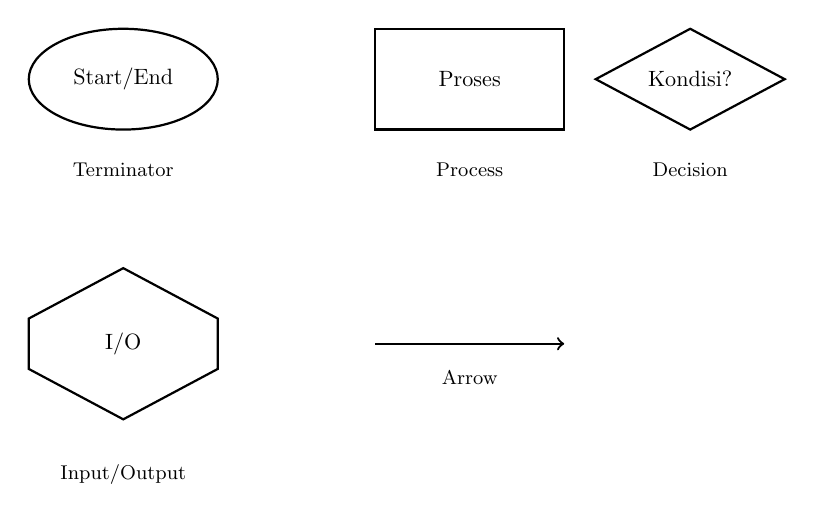
\begin{tikzpicture}[scale=0.8, transform shape]
  % Terminator
  \draw[thick] (0,0) ellipse (1.5cm and 0.8cm);
  \node at (0,0) {Start/End};
  \node[below] at (0,-1.2) {\small Terminator};
  
  % Process
  \draw[thick] (4,0.8) rectangle (7,-0.8);
  \node at (5.5,0) {Proses};
  \node[below] at (5.5,-1.2) {\small Process};
  
  % Decision
  \draw[thick] (9,0.8) -- (10.5,0) -- (9,-0.8) -- (7.5,0) -- cycle;
  \node at (9,0) {Kondisi?};
  \node[below] at (9,-1.2) {\small Decision};
  
  % Input/Output
  \draw[thick] (0,-3) -- (1.5,-3.8) -- (1.5,-4.6) -- (0,-5.4) -- (-1.5,-4.6) -- (-1.5,-3.8) -- cycle;
  \node at (0,-4.2) {I/O};
  \node[below] at (0,-6) {\small Input/Output};
  
  % Arrow
  \draw[thick, ->] (4,-4.2) -- (7,-4.2);
  \node[below] at (5.5,-4.5) {\small Arrow};
\end{tikzpicture}
\end{center}

\subsection{Aturan Penggunaan Simbol}

\begin{itemize}
  \item \textbf{Konsistensi:} Gunakan simbol yang sama untuk operasi yang sama di seluruh flowchart
  \item \textbf{Keterbacaan:} Pastikan teks di dalam simbol mudah dibaca dan singkat
  \item \textbf{Arah Alur:} Gunakan panah untuk menunjukkan arah alur yang jelas
  \item \textbf{Hierarki:} Simbol utama (terminator) selalu di bagian atas atau bawah
  \item \textbf{Koneksi:} Gunakan connector untuk flowchart yang kompleks
\end{itemize}

Pemahaman yang baik tentang simbol-simbol ini menjadi fondasi untuk membuat flowchart yang efektif dan sesuai standar industri.

\section{Membuat Flowchart Sederhana}

Untuk membuat flowchart, mulailah dengan simbol terminator bertuliskan "Mulai", kemudian tambahkan langkah-langkah algoritma secara berurutan menggunakan simbol proses atau input/output. Jika algoritma memiliki percabangan, gunakan simbol keputusan dengan dua cabang (Ya dan Tidak) yang menuju ke langkah yang sesuai. Akhiri flowchart dengan simbol terminator bertuliskan "Selesai". Pastikan setiap panah mengalir dengan jelas dan tidak ada langkah yang terputus.

\subsection{Contoh 1: Menentukan Bilangan Positif atau Negatif}

\textbf{Algoritma:}
\begin{enumerate}
  \item Mulai
  \item Input bilangan
  \item Jika bilangan > 0 maka tampilkan "Positif"
  \item Jika tidak maka tampilkan "Negatif"
  \item Selesai
\end{enumerate}

\textbf{Flowchart:}
\begin{center}
\begin{tikzpicture}[node distance=0.6cm]
  \node[flowstart] (start) {Mulai};
  \node[flowio, below=of start] (p1) {Input bilangan};
  \node[flowdecision, below=of p1] (d1) {bilangan > 0?};
  \node[flowprocess, below left=1.2cm of d1] (p2) {Tampilkan "Positif"};
  \node[flowprocess, below right=1.2cm of d1] (p3) {Tampilkan "Negatif"};
  \node[flowstart, below=2.5cm of d1] (end) {Selesai};
  \draw[arrow] (start) -- (p1);
  \draw[arrow] (p1) -- (d1);
  \draw[arrow] (d1) -| node[near start, above] {Ya} (p2);
  \draw[arrow] (d1) -| node[near start, above] {Tidak} (p3);
  \draw[arrow] (p2) |- (end);
  \draw[arrow] (p3) |- (end);
\end{tikzpicture}
\end{center}

\subsection{Contoh 2: Menghitung Rata-rata Tiga Bilangan}

\textbf{Algoritma:}
\begin{enumerate}
  \item Mulai
  \item Input bilangan1, bilangan2, bilangan3
  \item Hitung jumlah = bilangan1 + bilangan2 + bilangan3
  \item Hitung rata-rata = jumlah / 3
  \item Tampilkan rata-rata
  \item Selesai
\end{enumerate}

\textbf{Flowchart:}
\begin{center}
\begin{tikzpicture}[node distance=0.8cm]
  \node[flowstart] (start) {Mulai};
  \node[flowio, below=of start] (input) {Input bil1, bil2, bil3};
  \node[flowprocess, below=of input] (sum) {jumlah = bil1 + bil2 + bil3};
  \node[flowprocess, below=of sum] (avg) {rata = jumlah / 3};
  \node[flowio, below=of avg] (output) {Tampilkan rata};
  \node[flowstart, below=of output] (end) {Selesai};
  \draw[arrow] (start) -- (input);
  \draw[arrow] (input) -- (sum);
  \draw[arrow] (sum) -- (avg);
  \draw[arrow] (avg) -- (output);
  \draw[arrow] (output) -- (end);
\end{tikzpicture}
\end{center}

\subsection{Contoh 3: Loop untuk Menampilkan Bilangan 1-5}

\textbf{Algoritma:}
\begin{enumerate}
  \item Mulai
  \item Inisialisasi i = 1
  \item Jika i > 5 maka ke langkah 7
  \item Tampilkan i
  \item i = i + 1
  \item Kembali ke langkah 3
  \item Selesai
\end{enumerate}

\textbf{Flowchart:}
\begin{center}
\begin{tikzpicture}[node distance=0.8cm]
  \node[flowstart] (start) {Mulai};
  \node[flowprocess, below=of start] (init) {i = 1};
  \node[flowdecision, below=of init] (cond) {i > 5?};
  \node[flowio, below left=1.5cm of cond] (print) {Tampilkan i};
  \node[flowprocess, below=of print] (inc) {i = i + 1};
  \node[flowstart, below=2cm of cond] (end) {Selesai};
  \draw[arrow] (start) -- (init);
  \draw[arrow] (init) -- (cond);
  \draw[arrow] (cond) -| node[near start, above] {Tidak} (print);
  \draw[arrow] (print) -- (inc);
  \draw[arrow] (inc) |- (cond);
  \draw[arrow] (cond) -- node[near start, right] {Ya} (end);
\end{tikzpicture}
\end{center}

\subsection{Tips Membuat Flowchart yang Baik}

\begin{itemize}
  \item \textbf{Mulai dari atas:} Alur flowchart sebaiknya mengalir dari atas ke bawah
  \item \textbf{Gunakan simbol yang tepat:} Pastikan setiap operasi menggunakan simbol yang sesuai
  \item \textbf{Hindari persimpangan:} Usahakan garis alur tidak saling memotong
  \item \textbf{Label yang jelas:} Gunakan teks yang singkat namun jelas
  \item \textbf{Uji logika:} Pastikan flowchart merepresentasikan algoritma dengan benar
\end{itemize}

\section{Contoh Flowchart: Konversi Suhu}

Berikut contoh flowchart lengkap untuk mengonversi suhu dari Celsius ke Fahrenheit dengan implementasi dalam bahasa C.

\subsection{Algoritma Konversi Suhu}

\textbf{Algoritma:}
\begin{enumerate}
  \item Mulai
  \item Input suhu dalam Celsius
  \item Hitung Fahrenheit = Celsius $\times$ 9/5 + 32
  \item Tampilkan hasil Fahrenheit
  \item Selesai
\end{enumerate}

\subsection{Flowchart Lengkap}

\begin{center}
\begin{tikzpicture}[node distance=0.8cm]
  \node[flowstart] (start) {Mulai};
  \node[flowio, below=of start] (input) {Input Celsius};
  \node[flowprocess, below=of input] (calc) {F = C $\times$ 9/5 + 32};
  \node[flowio, below=of calc] (output) {Tampilkan F};
  \node[flowstart, below=of output] (end) {Selesai};
  \draw[arrow] (start) -- (input);
  \draw[arrow] (input) -- (calc);
  \draw[arrow] (calc) -- (output);
  \draw[arrow] (output) -- (end);
\end{tikzpicture}
\end{center}

\subsection{Implementasi dalam Bahasa C}

\begin{lstlisting}[language=C, caption={Program Konversi Suhu Celsius ke Fahrenheit}]
#include <stdio.h>

int main() {
    float celsius, fahrenheit;
    
    // Input suhu Celsius
    printf("Masukkan suhu dalam Celsius: ");
    scanf("%f", &celsius);
    
    // Konversi ke Fahrenheit
    fahrenheit = celsius * 9.0 / 5.0 + 32;
    
    // Tampilkan hasil
    printf("%.2f Celsius = %.2f Fahrenheit\n", celsius, fahrenheit);
    
    return 0;
}
\end{lstlisting}

\subsection{Analisis Karakteristik Algoritma}

\begin{itemize}
  \item \textbf{Input:} Satu nilai suhu dalam Celsius
  \item \textbf{Output:} Satu nilai suhu dalam Fahrenheit
  \item \textbf{Definiteness:} Langkah-langkah jelas (input, hitung, output)
  \item \textbf{Finiteness:} Algoritma berakhir setelah 4 langkah
  \item \textbf{Effectiveness:} Operasi aritmatika dasar dapat dilakukan
  \item \textbf{Determinism:} Input 25°C selalu menghasilkan 77°F
\end{itemize}

\subsection{Contoh Output Program}

\begin{verbatim}
Masukkan suhu dalam Celsius: 25
25.00 Celsius = 77.00 Fahrenheit

Masukkan suhu dalam Celsius: 0
0.00 Celsius = 32.00 Fahrenheit

Masukkan suhu dalam Celsius: 100
100.00 Celsius = 212.00 Fahrenheit
\end{verbatim}

Contoh ini menunjukkan bagaimana flowchart dapat membantu merancang algoritma sederhana sebelum implementasi dalam bahasa pemrograman.


\begin{aktivitas}
  \item Buat flowchart untuk menentukan bilangan ganjil atau genap.
  \item Buat flowchart untuk menghitung luas persegi panjang dari input panjang dan lebar.
  \item Buat flowchart untuk menampilkan bilangan 1 sampai 5.
\end{aktivitas}

\begin{latihan}
  \item Jelaskan fungsi masing-masing simbol flowchart: terminator, proses, keputusan, input/output!
  \item Buat flowchart untuk algoritma konversi suhu Celsius ke Fahrenheit!
  \item \textbf{Refleksi}: Apakah flowchart membantu Anda memahami alur algoritma? Jelaskan!
\end{latihan}

\begin{asesmen}
\textbf{Instrumen untuk Sub-CPMK 1.2}: Buat flowchart untuk menentukan nilai maksimum dari dua bilangan yang diinput.
\end{asesmen}

\begin{checklist}
  \item Saya dapat menjelaskan definisi dan fungsi flowchart
  \item Saya dapat mengenali simbol flowchart standar
  \item Saya dapat membuat flowchart untuk masalah sederhana
\end{checklist}

\begin{rangkuman}
Bab ini membahas flowchart sebagai representasi visual algoritma, simbol standar (terminator, proses, keputusan, input/output), dan cara membuat flowchart untuk masalah sederhana.
\end{rangkuman}

\ifSubfilesClassLoaded{
  \renewcommand{\bibname}{Daftar Pustaka}
  \bibliographystyle{plain}
  \bibliography{../references}
}{}
\end{document}
